\subsubsection{标注工具}
\textbf{labelImg介绍:}图片标注主要是用来创建自己的数据集,方便进行深度学习训练。本文使用labelImg
\begin{uscfigure}
	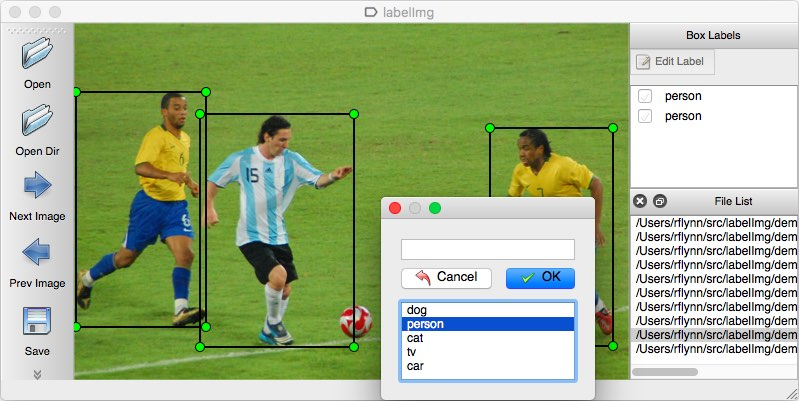
\includegraphics[width=\textwidth]{./Pictures/labelimg.jpg}	
	\caption{labelImg界面}
\end{uscfigure}
\subsubsection{数据集}
\textbf{VOC数据集介绍:}PASCAL VOC为图像识别和分类提供了一整套标准化的优秀的数据集。对于目标检测任务,我们只需要使用JPEGImage、Annotations、ImageSets三个文件夹。

其目录结构

- JPEGImage:文件夹包含了PASCAL VOC所提供的所有的图片信息,包括了训练图片和测试图片。

- Annotations:文件夹中存放的是xml格式的标签文件,每一个xml文件都对应于JPEGImages文件夹中的一张图片。

- ImageSet:存放的是每一种类型的challenge对应的图像数据。


\subsubsection{Pytorch介绍}
PyTorch是一个比较新的深度学习框架,正在研究人员中迅速普及。和深度学习框架Chainer类似,PyTorch支持动态计算图,这个功能使 PyTorch 对使用文本与时间序列的研究者和工程师很有吸引力。TensorFlow解决了质量控制和包装的问题。它提供了一种 Theano 风格的编程模式,所以它是一种非常底层的深度学习框架。由于TensorFlow本身是非常底层的框架,所以许多基于TensorFlow的前端框架应运而生,比如TF-slim和Keras。这样的框架目前有10到15个,仅Google就可能有四五个。

Torch的思想和Theano一直略有不同。TensorFlow是一个更好的Theano风格的框架,并且我们在Torch中注入了强制的思想,这意味着你可以立即运行你的计算。调试应该是平稳顺利的,用户在调试过程中不应当遇到难题,无论使用Python调试器还是像GDB或其他类似的东西。
\subsubsection{OpenCV介绍}
OpenCV是Intel\copyright 开源的计算机视觉库。它由一系列C函数和少量C++类构成 ,实现了图像处理和计算机视觉方面的很多通用算法。
\subsubsection{将图片切割成300px大小}
\begin{lstlisting}[caption={图像切割}]
img = img.resize(self.img_size, self.img_size)
\end{lstlisting}